\documentclass[titlepage, a4paper]{article}
\usepackage[english]{babel}
\usepackage[utf8]{inputenc}
\usepackage{graphicx}
\usepackage{color}
\usepackage{mathtools}
\usepackage{float}
\usepackage[parfill]{parskip}
\usepackage[margin=10pt,font=small,labelfont=bf,labelsep=endash]{caption}
\usepackage{epstopdf}
\usepackage{listings}
\epstopdfsetup{suffix=}
\DeclareGraphicsExtensions{.ps}
\DeclareGraphicsRule{.ps}{pdf}{.pdf}{`ps2pdf -dEPSCrop -dNOSAFER #1 \noexpand\OutputFile}

\lstset{literate=%
    {å}{{\r{a}}}1
    {ä}{{\"a}}1
    {ö}{{\"o}}1
    {Å}{{\r{A}}}1
    {Ä}{{\"A}}1
    {Ö}{{\"O}}1
}

\newcommand{\todo}[1] {\textbf{\textcolor{red}{#1}}}

\usepackage{fancyhdr}
\fancyhead[L]{}
\pagestyle{fancy}
\rhead{Alexander Yngve \\ Pål Kastman}
\chead{TDDC78}
\thispagestyle{empty}

\begin{document}

{\ }\vspace{45mm}

\begin{center}
  \Huge \textbf{TDDC78: Lab Report}
\end{center}
\begin{center}
  \Large Lab 4: Totalview \& ITAC
\end{center}

\vspace{250pt}

\begin{center}
  \begin{tabular}{|*{3}{p{40mm}|}}
    \hline
    \textbf{Name} & \textbf{PIN} & \textbf{Email} \\ \hline
           {Alexander Yngve} & {930320-6651} & {aleyn573@student.liu.se} \\ \hline
           {Pål Kastman} & {851212-7575} & {palka285@student.liu.se} \\ \hline
  \end{tabular}
 \end{center}
\newpage

\tableofcontents
\thispagestyle{empty}
\newpage


\section{Totalview}
Most of the time we write our code in Emacs, so we never use built-in debuggers as can be found in for some IDE:s, such as Eclipse. The only other debugger that we have tried out in previous courses before this one, is GDB. The most noticable difference between these two is of course that GDB is run from a terminal while Totalview is a graphical tool.

After fiddling with Totalview for a while we managed to get our source code visible in the debugger and setting breakpoints and running the program. The code contained no bugs that we were aware of, so we generated one by switching the operands of a subtracion as can be seen in listing \ref{lst:org} and \ref{lst:bug}.

\begin{lstlisting}[caption=Original code., label=lst:org, breaklines=true, language=c]
threshold_filter(data, xsize, yends[rank]-ystarts[rank], colmax, world_size);
\end{lstlisting}

\begin{lstlisting}[caption=Code with a bug in it., label=lst:bug, breaklines=true, language=c]
threshold_filter(data, xsize, ystarts[rank]-yends[rank], colmax, world_size);
\end{lstlisting}

The result of the bug is that the filter is not doing anything, which makes it logical to start debugging at the call to the filter. In figure \ref{fig:totview_breakpoint} a breakpoint has been set at the call to the filter. In figure \ref{fig:totview_variables} the debugger has entered the filter function where we can see that the argument ysize has a negative value causing the filter to never enter the its for-loop. The bug has been found!

\begin{figure}[H]
  \centering
  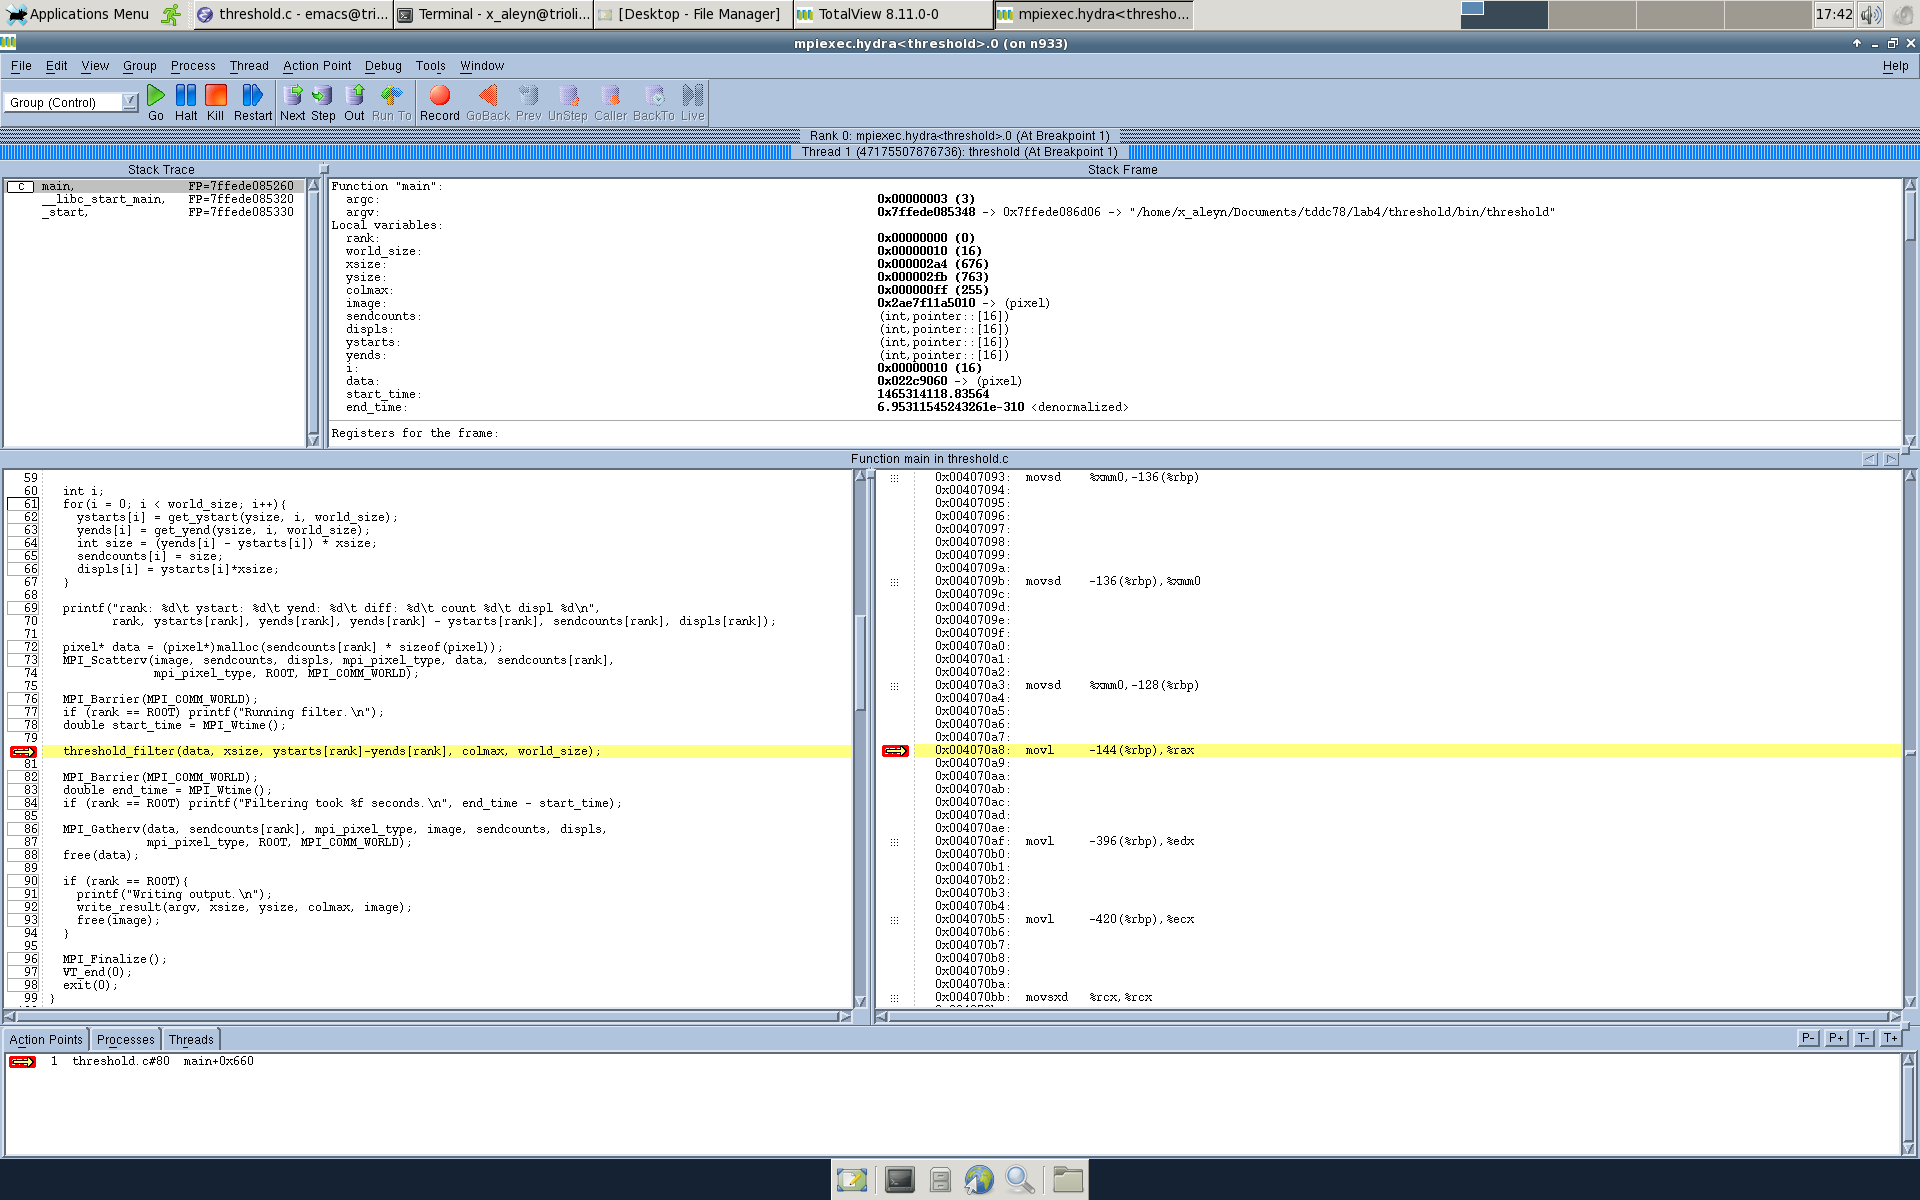
\includegraphics[scale=0.35, angle=90]{img/totview3.png}
  \caption{Setting a breakpoint at the call to the filtering function.}
  \label{fig:totview_breakpoint}
\end{figure}

\begin{figure}[H]
  \centering
  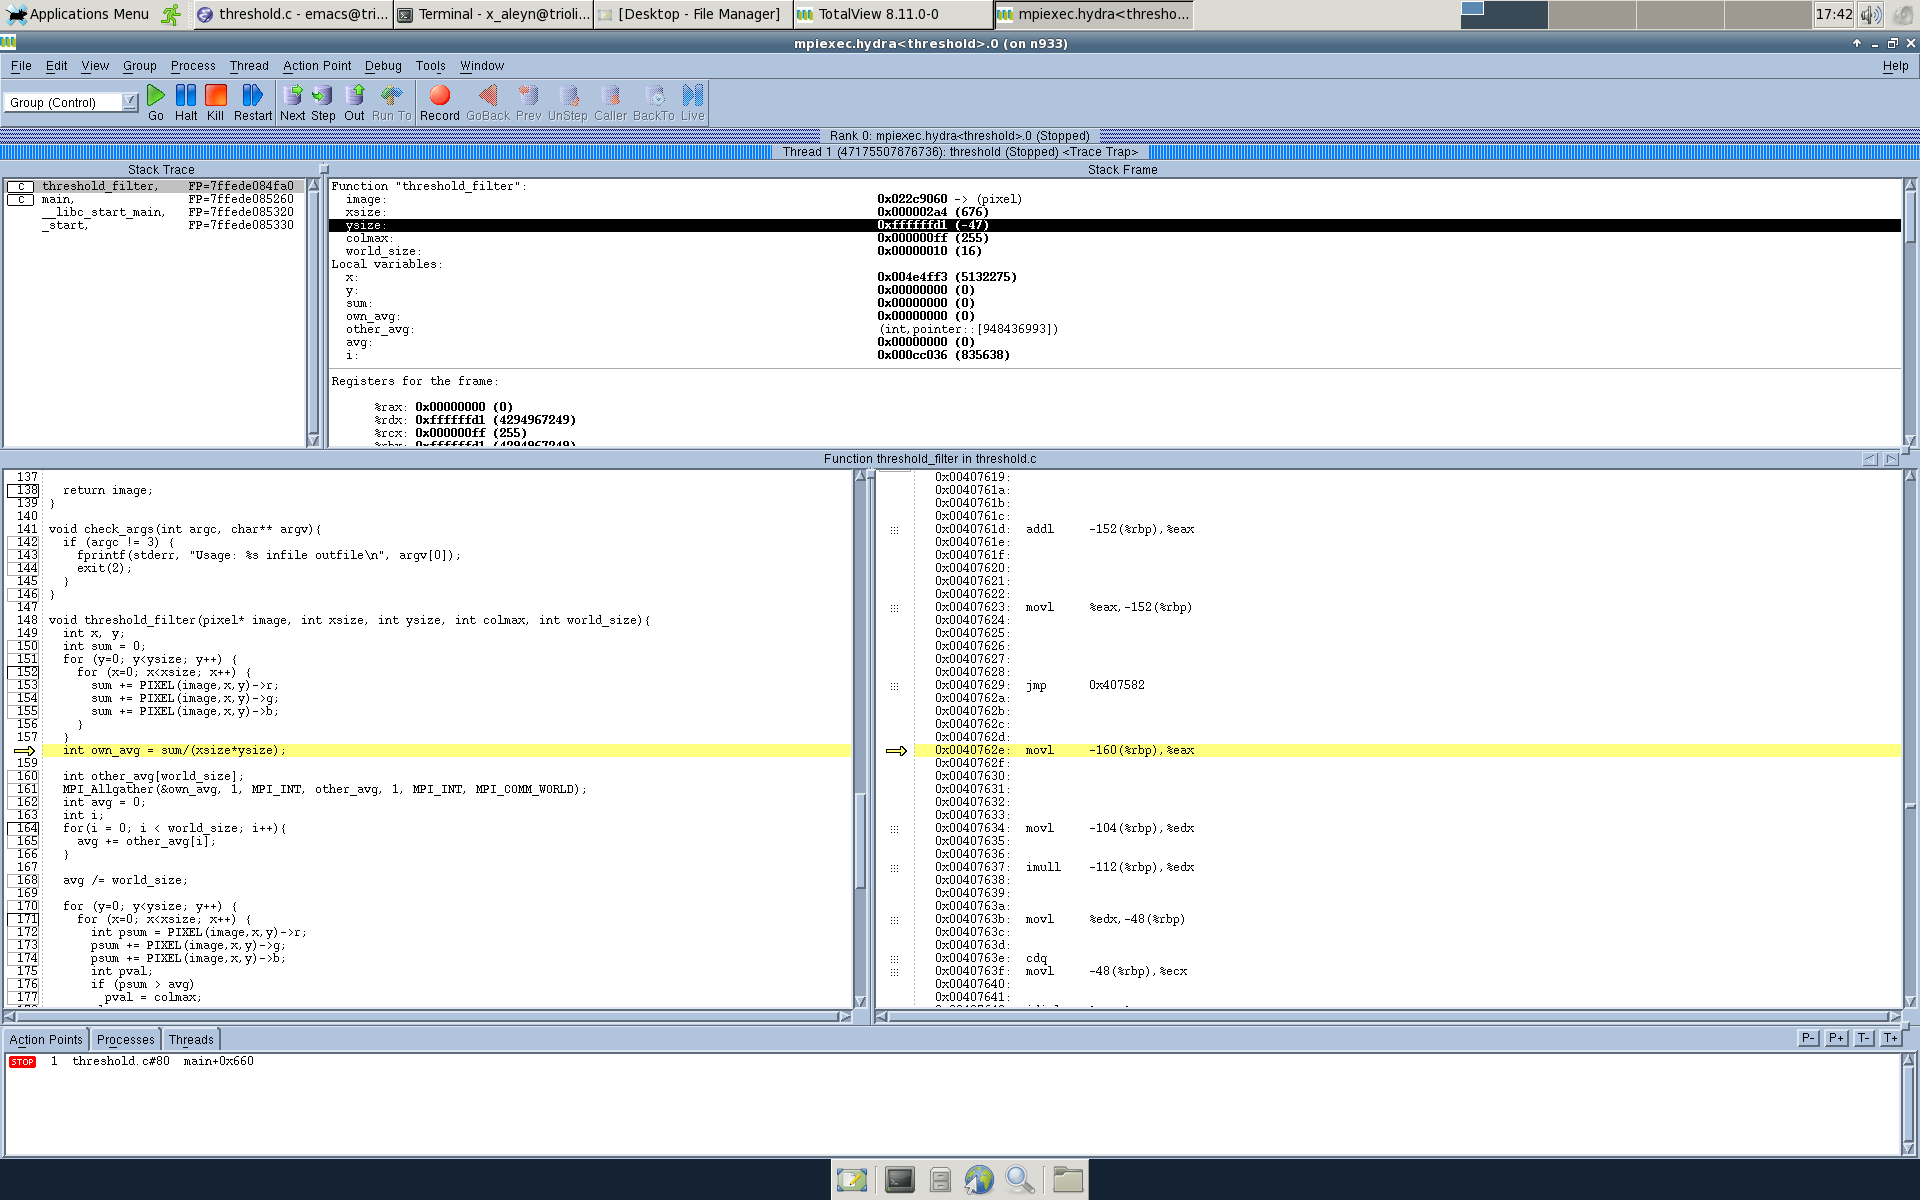
\includegraphics[scale=0.35, angle=90]{img/totview4.png}
  \caption{A faulty value found in the arguments to the filter.}
  \label{fig:totview_variables}
\end{figure}

\section{ITAC}
After a bit of trouble with compiling and linking our program with ITAC functions we finally got it to work. ITAC was quite straight forward to use and with ease we could see which functions in our program consumed the most time. This can be seen in figure \ref{fig:itac}. As can be seen no single function seem to be to time consuming. And the one that takes the most time is MPI\_Scatterv which can't be optimized further.

\begin{figure}[H]
  \centering
  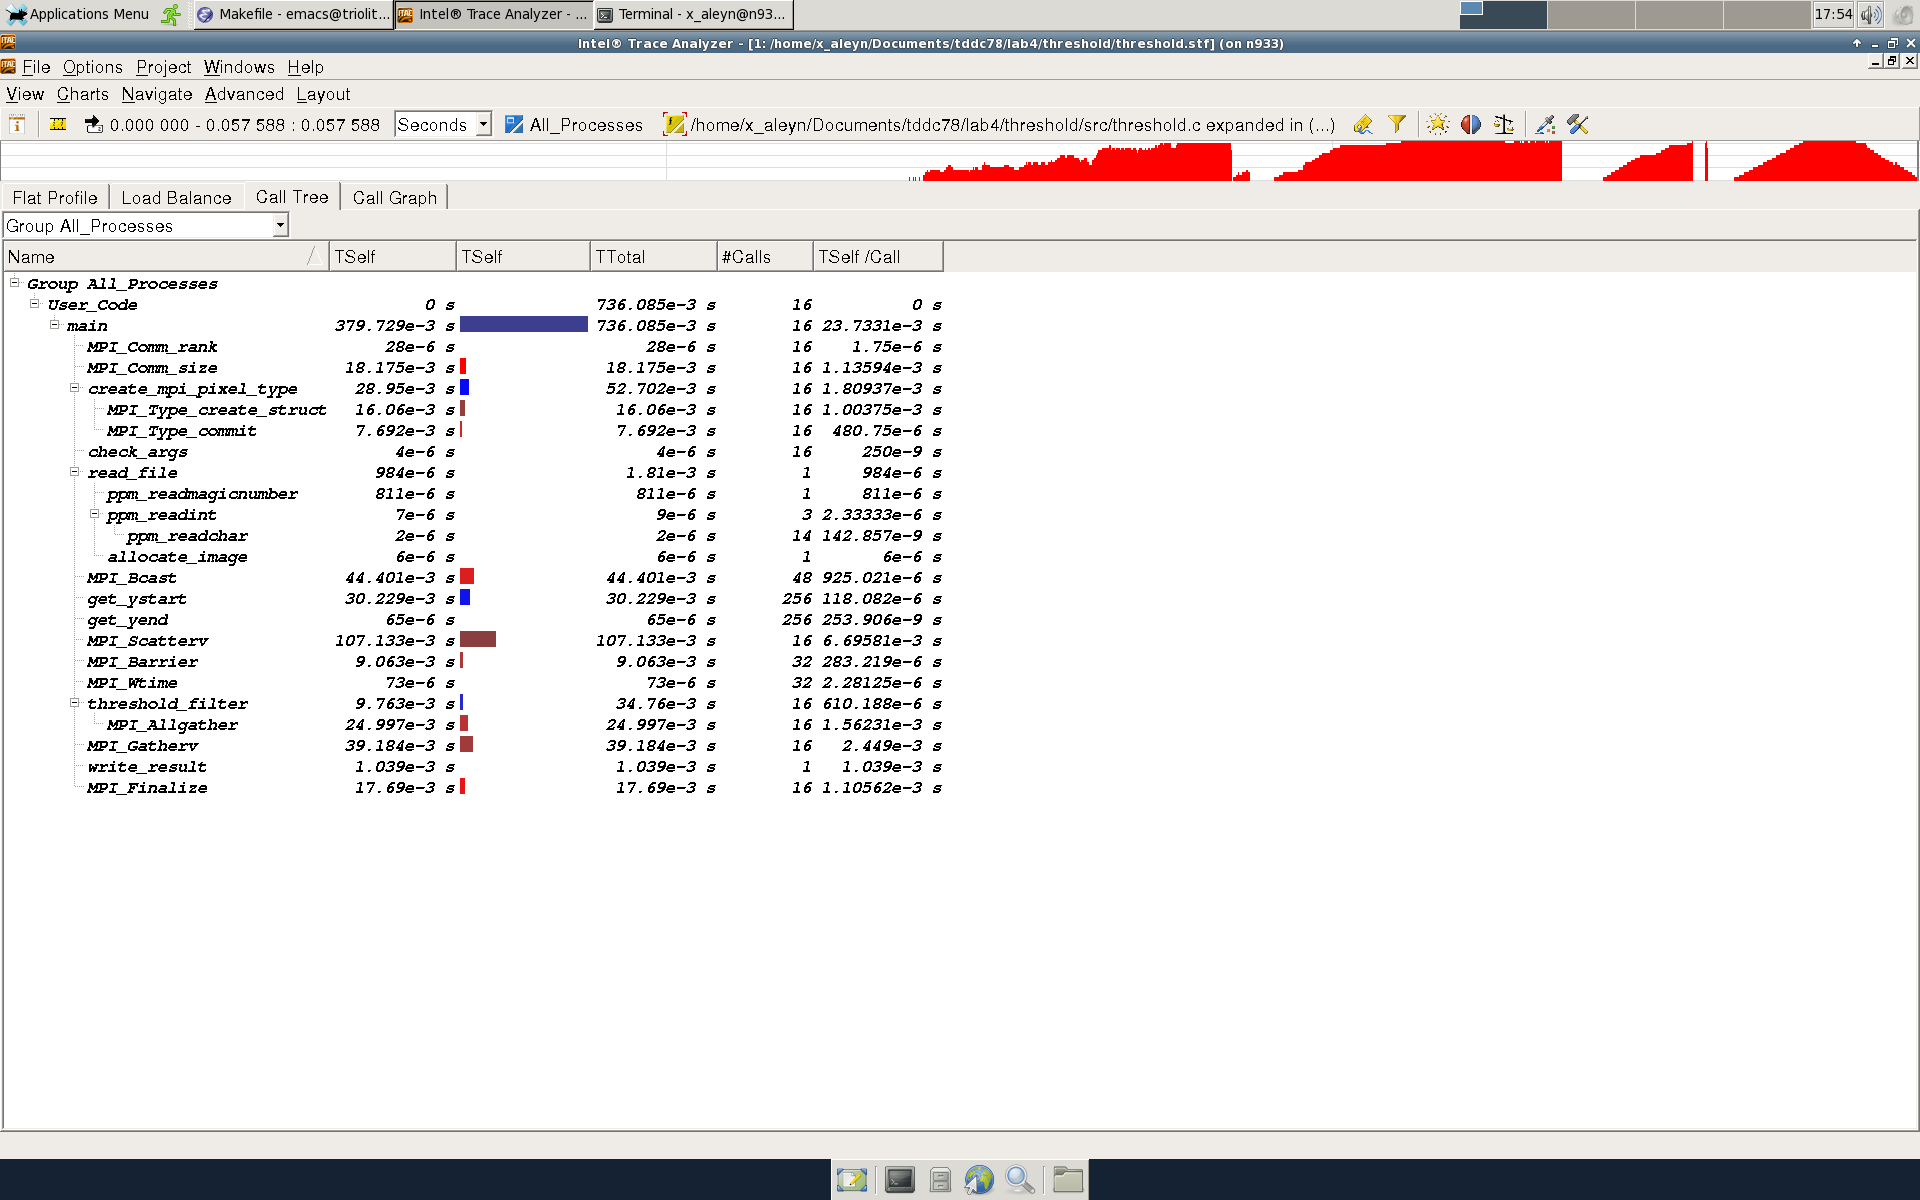
\includegraphics[scale=0.30, angle=90]{img/itac2.png}
  \caption{Intel ITAC.}
  \label{fig:itac}
\end{figure}

\section{Discussion}
Since using debuggers is quite a rare thing for us, Totalview felt very tricky to use. This is to be expected because Totalview is an advanced debugger, more advanced than GDB since it is specialized for multithreaded programs. However, when writing large parallel programs, we think it might be worth learning to use a debugger like Totalview, since a lot of bugs in parallel programs are very confusing and much harder to find than in serial programs.

ITAC on the other hand, was quite easy to use but a bit difficult to install and compile. Once you figured it out though it was a breeze. If you need to speed up your program and dont know where to start, it is definitely worth learning ITAC.
\end{document}
